
\documentclass{mpaper}
\usepackage{amsthm, esdiff}


\begin{document}
\newtheorem{lemma}{Lemma}
\newtheorem{theorem}{Theorem}
\newtheorem{conjecture}{Conjecture}
\theoremstyle{definition}
\newtheorem{definition}{Definition}
\newtheorem*{remark}{Remark}

\title{The Gilbert-Pollak Conjecture}
\author{Domonkos Revesz}
\matricnum{2480516r}

\maketitle

\begin{abstract}
According to Simon Peyton Jones, an abstract should address
four key questions. First, what is the problem that this
paper tackles? Second, why is this an interesting problem?
Third, what is the solution this paper proposes?
Finally, why is the proposed solution a good one?
\end{abstract}

\section{Introduction}

The idea of connecting various points in a network and producing a graph with the lowest possible cost has long been a subject of research in Mathematics and Computer Science. Examples include the minimum spanning tree, which describes the lowest possible cost graph on an undirected weighted graph; the travelling salesman problem, which describes the shortest cycle with all vertices in a graph and algorithms such as Dijkstra's also rely on such concepts. The Steiner tree is related to the minimum spanning tree; the difference between these two objects is that the Steiner tree can use vertices outside the set of vertices which must be in the minimum spanning tree, called \emph{Steiner points}.

One can calculate the minimum spanning tree in polynomial time, but the Steiner tree problem is proven to be NP-complete \cite{Pettie2008}. For large graphs, this means that the Steiner tree might take infeasibly long time to calculate, while the minimum spanning tree can be calculated efficiently. This poses a practical question: for a given graph $G$, is it worth to calculate the Steiner tree instead of the minimum spanning tree?

 In answering such a question, one has to answer the feasibility and cost of adding new vertices to the graph, the available computing power and the savings in cost that the Steiner tree can offer compared to the minimum spanning tree. The third criteria can be measured by the \emph{Steiner ratio} - the ratio between the minimum spanning tree and the Steiner tree for a given graph. Calculating the Steiner ratio involves calculating both the Steiner tree and the minimum spanning tree, and thus it does not save the expensive Steiner tree calculation. Instead, we can approximate the Steiner ratio by stating infimum and supremum of the Steiner ratio.
 
The supremum of the Steiner ratio is 1, because the Steiner tree cannot cost more than the minimum spanning tree. However, the infimum is not as obvious; it is different for different types of graphs. For graphs with arbitrary weights, the infimum does not exist - it is possible that all the vertices are connected to a single Steiner point with arbitrarily large absolute value weights with negative signs. If we restrict the weights, for example by embedding the points in an Euclidean plane, we get different infimum Steiner ratios. In 1976, F. K. Hwang \cite{doi:10.1137/0130013} showed that if the vertices are embedded in an Euclidean plane and the weights between the vertices correspond to their rectilinear distance, then the infimum and minimum Steiner ratio is $\frac{2}{3}$. Gilbert and Pollak conjectured in 1968 \cite{GP1968} if the vertices are embedded in an Euclidean plane and the weights between the vertices correspond to their Euclidean distance, then the infimum and minimum Steiner ratio is $\frac{\sqrt{3}}{2}$, achieved in the case of an equilateral triangle. Over the years, there have been several attempts made (\cite{doi:10.1073/pnas.87.23.9464}, \cite{myue}) to prove the conjecture, but none of the attempts survived intense scrutiny \cite{Ivanov2012}. This paper proposes two different approaches to this problem and provide discussion on previously used proof techniques.


\section{Notation and problem statement}

Let $S$ be a set of points, also called \emph{terminals}, in a Euclidean plane, i.e. each member of $S$ is a tuple $(x,y)$ where $x,y\in\mathbb{R}$. Let us define the weighted graph $G$, where the vertices of $G$ correspond to $S$, $G$ is complete graph, and the weight of edge $e$ between vertices $A$ and $B$ is defined as $w(e)=\operatorname{len}(e)$, where $len(e) = \sqrt{(x_A-x_B)^2+(y_A-y_B)^2}$. Furthermore, let us define $\operatorname{MST}(S)$ the minimum spanning tree of $G$. For the Steiner tree, we permitted to place at any coordinates; similarly to the terminals, each Steiner point must be connected to the rest of the points in $G$, including terminals and other Steiner points, and weights are defined the same way. Let us define $\operatorname{SMT}(S)$ to be the smallest cost Steiner tree of $G$. 
% By the \emph{topology} of $\operatorname{MST}(S)$ and . 
Let $\operatorname{len}(a,b)$ be the Euclidean distance between points $a$ and $b$; and let $\operatorname{L_S}(S)$ be the total cost of a SMT of S and let $\operatorname{L_M}(S)$ trees be the total cost of a MST of S.  Then, we can define the Steiner ratio of $S$ as
$$\operatorname{SR}(S)=\frac{\operatorname{L_M}(S)}{\operatorname{L_S}(S)}.$$


Finally, let us define \emph{cherry} as a Steiner point connected to at least two terminals and any amount Steiner points.
% \paragraph*{}


\section{History of the problem}
\subsection{Pre-Modern history}

The history of the conjecture stretches to back Fermat and Torricelli \cite{Brazil2014}, with only the special case of three points considered originally. Later, the generalized Fermat-Torricelli problem considered the case of $n$ points connected to a single point $S$ such that the sum of the sum of the length of the edges are minimized. The Euclidean Steiner tree problem was originally proposed and discussed by  the French mathematician Joseph Gergonne in 1810. Gergonne also proposed a general algorithm for finding the Steiner tree for $n$ points, which was later rediscovered by Melzak. This set forth a pattern of amnesia; the problem was subsequently discussed in various capacity by Gauss and Schumacher, who inspired two German mathematicians to investigate the problem restricted to four vertices, and was investigated by Czech mathematicians Jarník and Kössler and separately by the French mathematician Gustave Choquet; all of these groups seem to have been unaware of each other.

However, none of these studies formed the basis of modern discussion around Steiner trees; instead, the basis of the modern discussion is ascribed to the 1941 textbook \emph{What is Mathematics?: An Elementary Approach to Ideas and Methods}\cite{courant1996mathematics}. While it is a highly regarded textbook, it mistakenly states that the problem was proposed and developed by the German mathematician Jakob Steiner, who in truth had virtually no involvement with the problem; nevertheless, most modern treatments follow this erroneous nomenclature.

\subsubsection{Melzak (1961) \cite{melzak_1961}}
The first major publication on the subject of Steiner trees after \emph{What is Mathematics?} is Z.A. Melzak's paper on the construction of Steiner minimal trees. The paper lists 5 very basic properties of Steiner trees, one which is not proven. Then, it describes a brute force algorithm for constructing the exact Steiner minimum tree. By Melzak's own admission, the ``algorithm, although effective, is extremely redundant and inefficient''. While the paper's immediate practical impact was very low, it helped to set the terminology and directions of the field. Furthermore, in 1967,  E. J. Cockayne \cite{cockayne_1967}, a student of Melzak improved the algorithm, provided more complete version of Melzak's proofs and discussed the Steiner problem in other spaces and metrics.
\subsubsection{Gilbert and Pollak (1968) \cite{GP1968}}
This seminal paper is usually regarded as the theoretical basis for the majority of the following literature on Euclidean Steiner trees. Its original intent is to improve on Melzak's algorithm by identifying important geometric features and thus discarding a large chunk of possibilities. Firstly, it describes three kinds of trees: relatively minimal trees, Steiner trees and Steiner minimal trees. By establishing a hierarchy between these three kind of trees, it solidifies the theoretical basis for Steiner minimal trees and makes the following discussion easier.The established geometric properties include:
\begin{itemize}
\item Let $S$ be a Steiner tree, with vertices $A$, $B$ and $C$ and edges $AB$ and $BC$; then $\measuredangle ABC\geq120°$.
\item Every Steiner point of a Steiner tree has exactly three lines meeting at 120°.
\item Let $S$ be a Steiner tree on $n$ terminals; then the maximum number of Steiner points in $S$ is $n-2$. If $S$ has $n-2$ Steiner points, then it is a \emph{full Steiner tree}.
\item Let $S$ be a relatively minimal tree; then all Steiner points lie inside convex hull of the terminals of $S$.
\item Every non-full Steiner tree can be decomposed into a union of full Steiner trees by replacing each terminal $A_i$ having $k\geq 2$ neighbours by $k$ new terminals $A_{i1},\dots,A_{ik}$ all located at $A_i$ all connected to exactly one neighbour of $A_i$, but disconnected from each other.
\item For all sets of 3 terminals, the Steiner ratio is more than or equal to $\frac{\sqrt{3}}{2}$.
\end{itemize}

It also establishes an algorithm for Steiner minimal tree and enumerates the number of Steiner tree topologies on $n$ terminals and $k$ Steiner points. To reduce the number of possibilities, it lists several further properties of minimal trees which already satisfy the already-mentioned conditions, including:
\begin{itemize}
\item The lune property, which describes a vesica piscis-shaped region where no edges or vertices of Steiner tree can appear; this property also applies to minimum spanning trees.
\item The wedge and double wedge properties, which restrict the edges of Steiner trees.
\item The distance property, restricts the length of edges between two Steiner points.
\item The diamond property, which constructs a rhombus for each edge in a minimal tree; the property posits that none of these rhombi can overlap.
\item Deciding regions, which expand on the lune property for Steiner trees.
\end{itemize}

Finally, the paper conjectures the minimum Steiner ratio as $\frac{\sqrt{3}}{2}$, but does not prove it. However, it proves a much lower minimum Steiner ratio as $\frac{1}{2}$. % It also posits an argument similar to Lemma \ref{ft}; however, they are not exactly the same.

To help illustrate some properties and prove others, the paper describes an analogous concept, ``a mechanical system in which the potential energy is a sum of distances between adjacent vertices''. The paper never rigorously proves that this system is equivalent to Steiner trees, although it cites other papers in which similar networks are described. For people trained in classical physics, this formulation might be self-evident; however, by today's standards this would not count as scientifically accurate.


\subsubsection{Pushing the lower bound}
\textbf {R.L. Graham and F. K. Hwang} \cite{1/sqrt3} proved in 1976 that $\operatorname{SR}(S)\geq\frac{1}{\sqrt{3}}$, for any set of points $S$ in an $n$-dimensional Euclidean space; the 2-dimensional Euclidean space is also called an Euclidean plane.  The paper's approach is that it assumes a full Steiner tree and then analyses a cherry. Unlike the following papers, the papers only focuses on one lower bound, without trying to combine multiple conditions. While the result does not push the minimum by a large amount, the proof is very short and does not use any advanced mathematics; however it skips a few steps, which makes it hard to understand. It is clear that this proof was intended to be a stepping stone, rather than a final conclusion. 

\textbf{F. R. K. Chung and F. K. Hwang} \cite{3a161666-bf4c-3db7-b5bc-795aa21aed1b}  in 1978 improved the lower bound to $0.74309\dots$. The paper's approach is similar to \cite{1/sqrt3}; it also analyses a cherry but it picks multiple conditions instead of a single condition to rule out vertices at different positions. This paper highlights one of the advantages of today compared to 1978: even this proof involved a large amount of manual calculations, which took a lot of time calculate; this made it hard to explore different conditions. Nonetheless, this paper is a lot more mature than \cite{1/sqrt3}.

\textbf{D. Z. Du and F. K. Hwang} \cite{d6ebcb0d-eded-3f80-b57b-cda0b84fa6c0} raised the lower bound to 0.8 in 1983. Like the last two proofs, this also focuses on cherries, and like \cite{1/sqrt3}, it mostly focuses on one condition, which is not used here. Nevertheless, this approach was promising, but its development was cut short by the following two papers.
% present an overview of relevant previous work including articles, books, and existing software products. Critically evaluate the strengths and weaknesses of the previous work.

Finally, \textbf{F. Chung and R. Graham} \cite{finalb} improved the lower bound to $0.824\dots$ in 1985. The proof uses induction; on a deeper level, the induction step is adding two points to form a cherry.  This is very similar to our approach, but instead we take away the terminals of the cherry, and use different conditions. Compared to the previous papers, it uses machine calculations instead of manual solving. Notably, it is explicitly verbose because ``on more than one occasion in the past, [...] proofs of bounds for this problem have proven to be incorrect'', which is in stark contrast with the following paper.

\subsubsection{D. Z. Du and F. K. Hwang (1992) \cite{doi:10.1073/pnas.87.23.9464}}
This paper claims to have solved the Gilbert-Pollak Conjecture; unlike the previous  attempts, this paper proposes a brand-new approach: instead of looking at any specific substructures found within Steiner trees, it tries to argue about the general structure of the whole graph. This makes the approach more appealing than the previous approaches, as it uses little Euclidean geometry and thus easier to generalize to other distance metrics and other kinds of topological spaces (such as curved surfaces). However, it was later discovered that this proof has gaps which cannot easily be rectified \cite{Ivanov2012}, and nobody has resolved these gaps up to this day.


The most important objects in the proof are the characteristic area of Steiner trees and their associated inner spanning trees. The characteristic area of a Steiner tree is a convex polygon which contains all the edges and vertices of the given Steiner tree. This area, however, is not necessarily planar; it can also be a manifold. The inner spanning tree is a minimum spanning tree which fully lies inside the characteristic area. The paper argues that the smallest cardinality set of points $S$ such that $\operatorname{SR}<\frac{\sqrt{3}}{2}$ has an inner spanning tree, and the length of the inner spanning tree is less than $\frac{2}{\sqrt{3}}\operatorname{SR}$, and thus arrives at a contradiction.

In his PhD thesis, P. O. De Wet \cite{po} criticizes this and related papers written by Du-Hwang on the grounds that several objects and inner spanning trees in particular are not rigorously defined. Furthermore, he shows that inner spanning trees does not have an obvious definition which satisfies all required properties mentioned in the Du-Hwang paper, and thus the Gilbert-Pollak conjecture is still open. Nevertheless, he gives a rigorous definition of inner spanning trees and proves the conjecture for 7 points, but notes that a general proof would need some more work.


% This section will detail the various empirical evidence in support of the conjecture and proposes the first half of a proof that according to empirical results might be able the resolve the conjecture. Firstly, experiments using random graphs and machine learning will demonstrate that the conjecture in the average case usually holds. Then, something

\section{Empirical analysis} \label{sec:ea}

\begin{figure}
  \begin{center}
  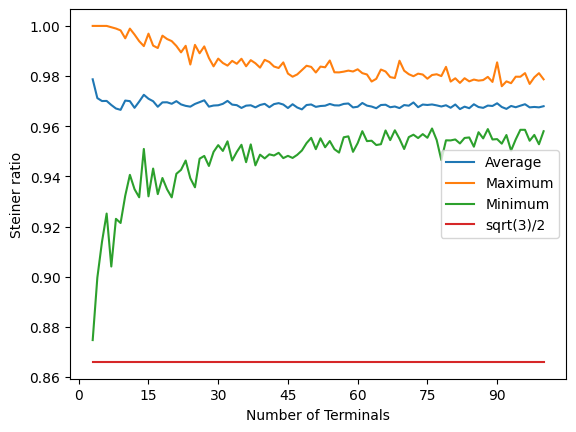
\includegraphics[scale=0.5]{plot2.png}
  \end{center}
  \caption{\label{fig:1}Description of the Steiner ratio on 3 to 100 terminals; each number of terminals was generated 100 times, and the Steiner trees were generated by the GeoSteiner algorithm. Each point was uniformly generated in ([0;1], [0;1]). }
\end{figure}

  \begin{figure}
    \begin{center}
    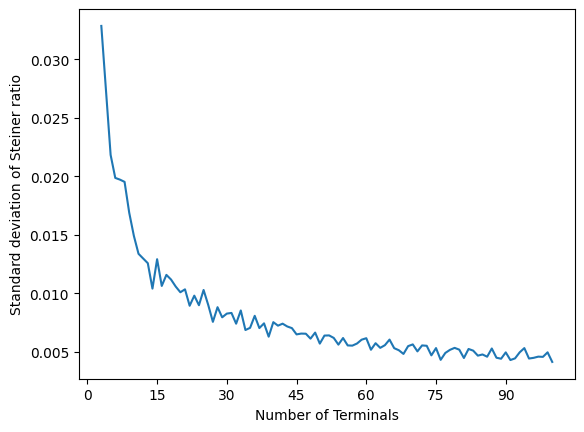
\includegraphics[scale=0.5]{plot3.png}
    \end{center}
    \caption{\label{fig:3} The standard deviation for each terminal from Figure \ref{fig:1}}
\end{figure}
  
\begin{figure}
  \begin{center}
  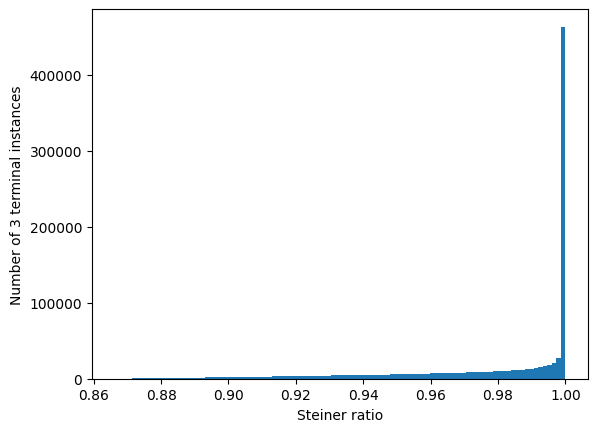
\includegraphics[scale=0.5]{plot4.png}
  \end{center}
  \caption{\label{fig:4} The Steiner ratio of 1000000 3 terminal instances, separated into 100 bins. Each point was uniformly generated in ([0;1], [0;1]).}
\end{figure}



\begin{figure}
  \begin{center}
  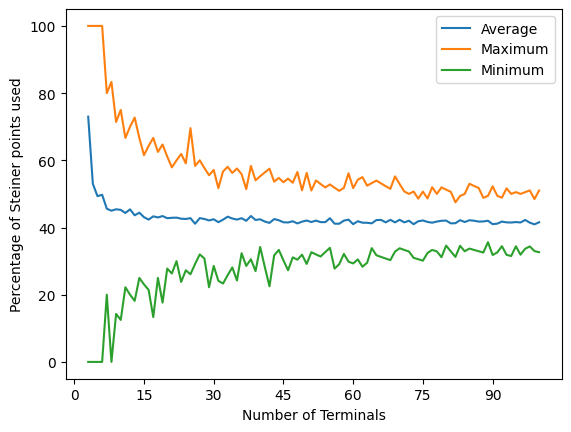
\includegraphics[scale=0.5]{plot1.png}
  \end{center}
  \caption{\label{fig:2}Description of the percentage of Steiner points used on 3 to 100 terminals; each number of terminals was generated 100 times, and the Steiner trees were generated by the GeoSteiner algorithm. Each point was uniformly generated in ([0;1], [0;1]). }
\end{figure}

\begin{figure}
  \begin{center}
  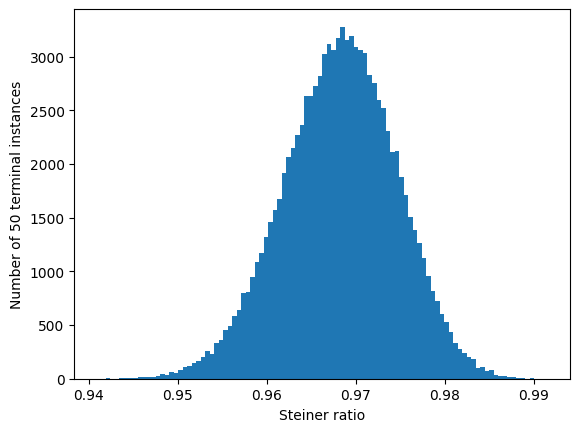
\includegraphics[scale=0.5]{plot5.png}
  \end{center}
  \caption{\label{fig:5} The Steiner ratio of 100000 50 terminal instances, separated into 100 bins. Each point was uniformly generated in ([0;1], [0;1]).}
\end{figure}

\begin{figure}
  \begin{center}
  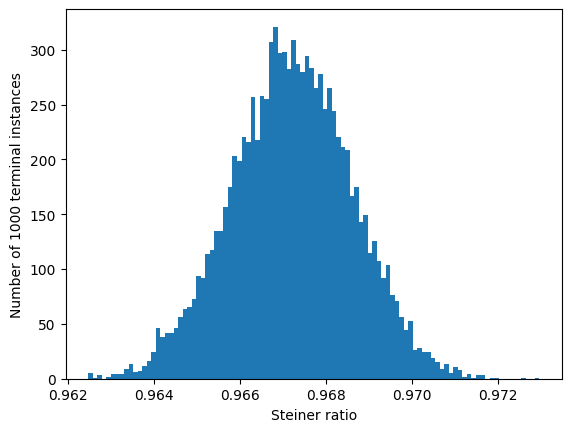
\includegraphics[scale=0.5]{plot6.png}
  \end{center}
  \caption{\label{fig:6} The Steiner ratio of 10000 1000 terminal instances, separated into 100 bins. Each point was uniformly generated in ([0;100], [0;100]).}
\end{figure}

 Gilbert and Pollak \cite{GP1968} give us the expected Steiner ratio on 3 terminals using three methods of terminal construction, while Pollak \cite{POLLAK1978278} reports that ``experiments by Gilbert indicate a typical shortening, for random points, of perhaps 2 to 3\%''. In this section, we will analyse various set of randomly generated terminals to give us an understanding of the average case usefulness of the Steiner tree. Each of the coordinated sets of terminals were generated by a uniform distribution from the interval $[0;1]$ (except where otherwise noted). We generate the minimum spanning trees using Prim's algorithm implemented in C, and we generate the Steiner minimum tree using the GeoSteiner algorithm.

Figure \ref{fig:1} shows the Steiner ratios of randomly generated points. The mean converges to roughly 0.967,  which is in line with the observation made by Gilbert; the minimum and maximum also converges to this number. No instance was found to have violated the conjecture; in fact, no random instance reached even the conjectured limit. This suggests that the conjecture is true and that this way of randomly generating points does not yield a low Steiner ratio. Furthermore, the global minimum is reached in the minimum amount of terminals (i.e. three terminals), and the minimums exhibit an increasing trend from that point on. Nonetheless, the global maximum also occurs at three terminals; as Figure \ref{fig:3} shows us, the standard deviation also decreases as we increase the number of terminals.

In other words, Steiner trees are able to save the most on three terminals if the terminals are adequately placed; however, three terminals are also the most likely to have a Steiner ratio of 1. We hypothesize that as we increase the number of terminals, we also increase the number of triangles we put down, and thus we repeat (or sample) the experiment on three terminals inside the higher terminal instances. As Figure \ref{fig:4} shows us, the distribution of Steiner ratios on 3 terminals is heavily negatively skewed; thus, we are more likely to get high Steiner ratio triangles in high number of terminals as well. If this is indeed the case, then we should expect the distribution of the Steiner ratios of the higher terminal instances to be normal because of the Central Limit Theorem. Figure \ref{fig:5} tentatively confirms this; while the distribution is skewed negatively and the D'Agostino and Pearson's normality test reports a p-value of 7.4e-87, i.e. it is statistically very unlikely that it is drawn from a normal distribution, visually it looks very similar to a normal distribution; perhaps, we need to test it with even more terminals. The data from Figure \ref{fig:6} has a much higher p-value of 0.437, validating our hypothesis.

Nevertheless, the measured mean (0.967) is lower than what we would expect based on the mean of the data presented in Figure \ref{fig:4}, which is 0.980. This might be explained by 4 and higher terminal full Steiner trees being more likely to form as we increase the number of terminals. 

TODO: Maybe a paragraph about generating in rectangles?

\section{Machine learning and real analysis}


In the previous section, we looked at the average-case scenarios, however we did not at the worst case (meaning instances where the Steiner ratio is the lowest possible). To find out such instances, we could try to use optimizers to learn more about these instances. Firstly, we define the domain as $n\mathbb{R}^{2}$, where $n$ is the number of terminals, and thus $\{\{x_1, y_1\}, \{x_2, y_2\} \dots \{x_n, y_n\}\}$ are the $x$ and $y$ coordinates of the terminals; let $S=\{s_1, s_2, \dots s_n\}$ denote the associated set of terminals, and then we can define the loss function as $\operatorname{SR}(S)$. To ensure that the loss function can be optimized well, we have to show that it is continuous and differentiable in most places.

\begin{lemma}
  \label{l:2}
  $\operatorname{SR}$ is continuous at almost all values of the domain and differentiable and twice differentiable at some values of the domain for all $n$.
\end{lemma}
\begin{proof}
  To prove this statement, we need to prove that both $\operatorname{L_S}$ and $\operatorname{L_M}$ is continuous.

  Let us use the notation as defined above; firstly, to prove that $\operatorname{L_M}$ is continuous at almost all values of the domain, we only need to prove  that $\operatorname{L_M}$ is continuous at all possible $x_1$, if all other coordinates are fixed. This is because the ordering of the terminals in the input does not matter (i.e. $\operatorname{L_M}(\{\{1,2\}, \{3,4\}, \{5,6\}\})=\operatorname{L_M}(\{\{5,6\}, \{1,2\}, \{3,4\}\}))\\$ and the length of the minimum spanning tree is preserved under 90° rotation (i.e. $\operatorname{L_M}(\{\{1,2\}, \{3,4\}, \{5,6\}\})=\\\operatorname{L_M}(\{\{2,1\}, \{4,3\}, \{6,5\}\})$).

  There are two cases for $s_1$ in the minimum spanning tree; $s_1$ can be in a breakpoint where if we change $x_1$ we get two different minimum spanning tree topologies depending on the direction of the change or $s_1$ is not in a breakpoint, meaning changing the coordinate either way will result in the same topology.

  If $s_1$ is not in a breakpoint, then $\operatorname{L_M}$ is continuous in $s_1$ because we are only changing the length of one edge in the minimum spanning tree; if we assume wlog that $s_1$ is connected to $s_2$ and $x_1'$ is the new $x$ coordinate of $s_1$, then the new weight of the minimum spanning tree is
  
  \begin{equation}
    \label{eq:3}
  -\sqrt{(x_1-x_2)^2 + (y_1-y_2)^2} + \sqrt{(x_1'-x_2)^2 + (y_1-y_2)^2}
  \end{equation}

  which is a composition of continuous functions and thus is continuous. Furthermore, this is a composition of differentiable and twice differentiable functions on almost all places, except where $(x_1'-x_2)^2 + (y_1-y_2)^2 =0$ (i.e. where two terminals have the same coordinate). 

  If $s_1$ is in a breakpoint, then it must be both right and left continuous. Wlog let us assume it is not left continuous; meaning the limit of the left topology has a larger limit at $s_1$ than the right topology; this cannot happen, because then we could produce a minimum spanning tree by using the right topology instead of the left topology. However, $\operatorname{L_M}$ is not guaranteed to be differentiable at breakpoints.

  % because as we are continuously change the coordinate of $S_1$, we only change one edge in the 

  For $\operatorname{L_S}$, we can repeat the same argument.
  % Suppose $\operatorname{L_S}$ is discontinuous at $x_1$, meaning that (using the $\epsilon-\delta$  definition of continuity) there is an $\epsilon$ such that we cannot find a $\delta$ that satisfies the continuity condition. In other words, there exists a terminal $s_1$ such that if we change the $x$ coordinate, $\operatorname{L_S}$ performs a sudden jump. 

  % Similar to the breakpoint argument for $\operatorname{L_M}$, this cannot happen because then we could produce a Steiner tree with lower cost on the higher side of the discontinuity by constructing the Steiner tree on the lower side of the discontinuity and treating the terminal  $s_1'$ as a Steiner point and connecting it to the position of the terminal on the higher side. TODO: This is a bit unclear, maybe ask Yiannis.

  Thus, because the quotient of two continuous functions are continuous (expect where the denominator is 0, i.e. the instances where all terminals have the exact same coordinates), the $\operatorname{SR}$ function is continuous. Moreover, on places where both $\operatorname{L_M}$ and $\operatorname{L_S}$ does not have any overlapping terminals or overlapping terminals and Steiner points and both $\operatorname{L_M}$ and $\operatorname{L_S}$ does not have breakpoints, $\operatorname{SR}$ is differentiable and twice differentiable.

  % Suppose there exists a set of points $T$ such that $\operatorname{L_S}(T)$ or $\operatorname{L_M}(T)$ is discontinuous. This means that 
\end{proof}

\begin{conjecture}
  $\operatorname{SR}$ is differentiable and twice differentiable at almost all values of the domain for every $n$.
\end{conjecture}

% (TODO: maybe prove it? we prove continuity for global minima later, this is not really relevant) 

If this indeed holds, then optimizers should be able to lower the Steiner ratio successfully. Figure \ref{fig:7} demonstrates that some optimizers can indeed be used to find instances with low Steiner ratios; if we accept the conjecture, then they are able to find instances with the global minimum Steiner ratio. Naturally, no instances were found with Steiner ratio less than $\frac{\sqrt{3}}{2}$. (TODO: maybe add more instances and demonstrate this claim?) In the instance of Figure \ref{fig:7}, the optimization process yielded 4 equilateral triangles, however the optimizer can get trapped in local minima, as Figure \ref{fig:8} demonstrates. After repeating the optimization process 100 times with a different set of random points in each run, we get a mean Steiner ratio of 0.870.


\begin{figure}
  \begin{center}
  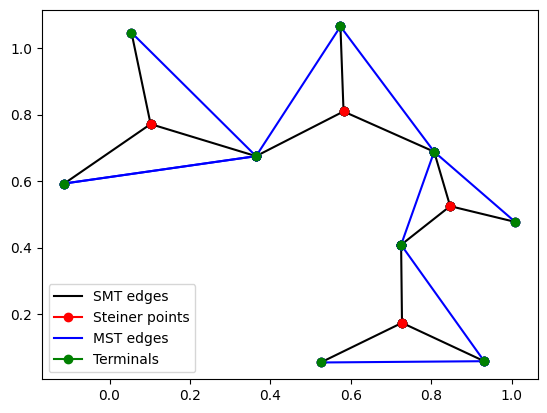
\includegraphics[scale=0.5]{plot7.png}
  \end{center}
  \caption{\label{fig:7}10 random points optimized for $\operatorname{SR}(S)$ with SLSQP; $\operatorname{SR}(S)=0.866\dots\approx\frac{\sqrt{3}}{2}$}
\end{figure}

\begin{figure}
  \begin{center}
  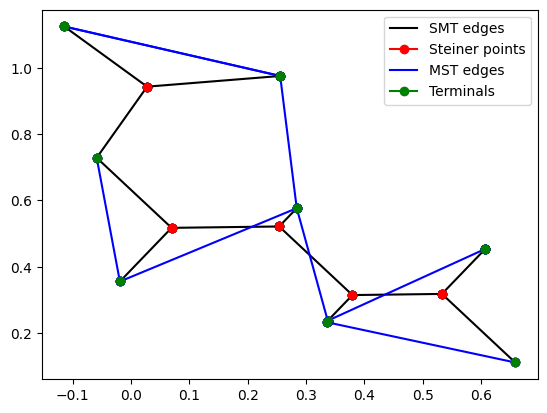
\includegraphics[scale=0.5]{plot8715.png}
  \end{center}
  \caption{\label{fig:8}10 random points optimized for $\operatorname{SR}(S)$ with SLSQP; $\operatorname{SR}(S)\approx 0.8715$}
\end{figure}

\subsection{Local minima}

As Figure \ref{fig:8} and \ref{fig:9} demonstrates, the optimizer was not able to find the hypothesized global minimum in all cases, because it got stuck in local minima. From these examples, we can extrapolate properties of local minima and thus global minima of the Steiner ratio function.

In every exhibited case, the minimum spanning tree is not unique - i.e. it is in a breakpoint. Intuitively, this is because if we slide the terminals along the Steiner tree edge, we change the length of the Steiner edge and thus the weight of the Steiner tree linearly. If we increase the Steiner edge, then we only increase one edge in the minimum spanning tree, and this increase is less than or equal to the increase of the Steiner edge. If we decrease the Steiner edge, then we decrease two edges in the minimum spanning tree, and this decrease is more than or equal to the decrease of the Steiner edge. Figure \ref{fig:10} demonstrates this. Thus, 

\begin{lemma}
  \label{l:1}
  Let $n$ be the number of terminals and let $S$ be an input vector for $\operatorname{SR}$. $\operatorname{SR}(S)$ is a local minimum if every terminal is in a breakpoint.
\end{lemma}
\begin{remark}
  Let $f'(x)$ denote the derivative of $f(x)$, and let $f'(x^+)$ and $f'(x^-)$ denote the right-hand side and left-hand side derivatives of $f(x)$, respectively.

  Breakpoint here is used in the same sense as in the proof of Lemma \ref{l:2}.
\end{remark}
\begin{proof}
  Let $S$ be a set of terminals such that $SR(S)$ is a local minimum; this means that if we fix every coordinate but $x_1$, we get an $\mathbb{R}\rightarrow \mathbb{R}$ function that has a local minimum at $x_1$; let us name this function 
  
  $$\operatorname{SR^1}(x)=\frac{\operatorname{L_S^1}(x)}{\operatorname{L_M^1}(x)}$$
  
  Without loss of generality, let us assume that the Steiner edge connected to $s_1$ is parallel to the $x$ axis and the Steiner point connected to $s_1$ has a lower $x$ value than $s_1$ (e.g. Steiner point connected to $s_1$ is left of $s_1$); we can do this because length of both trees are preserved under rotation. This way, as we change $x$ from $x_1$, $\operatorname{L_S^1}(x)$ changes by the same amount, i.e. $\operatorname{L_S^1}'(x_1)=1$. Furthermore, it is enough to only examine $x_1$ for the same reasons as detailed in the proof of Lemma \ref{l:2}.

  Because we are in a local minimum, as we increase $x$ from $x_1$, $\operatorname{SR_1}(x)$ must also increase. This is only the case if the minimum spanning tree increases less than the Steiner ratio is at $x_1$, i.e.
  \[
    \operatorname{L_M^1}'(x_1^+)\leq\operatorname{SR^1}(x_1)
  \]
  Similarly from the left side:
  \[
    \operatorname{L_M^1}'(x_1^-)\geq\operatorname{SR^1}(x_1)
  \]

  In other words, $\operatorname{L_M^1}'$ must be decreasing at $x_1$. Let us now calculate the first and second derivative of $\operatorname{L_M^1}(x)$ if $x$ is not in a breakpoint using Equation \ref{eq:3} and using $x$ instead of $x_1'$:
  \begin{eqnarray}
    \operatorname{L_M^1}'(x) =\dfrac{x-x_2}{\sqrt{\left(x-x_2\right)^2+\left(y_1-y_2\right)^2}}\\
    \operatorname{L_M^1}''(x) =\dfrac{\left(y_1-y_2\right)^2}{\left(\left(x-x_2\right)^2+\left(y_1-y_2\right)^2\right)^\frac{3}{2}}  
  \end{eqnarray} 
  If $x$ is not a breakpoint and the resulting set of terminals does not have any overlaps, then $\operatorname{L_M^1}''(x)\geq 0$; this means that  $\operatorname{L_M^1}'(x)$ is a monotone increasing function. This means that $\operatorname{L_M^1}(x)$ must be in a breakpoint, proving our original statement.
\end{proof}

\begin{figure}[h!]
  \begin{center}
  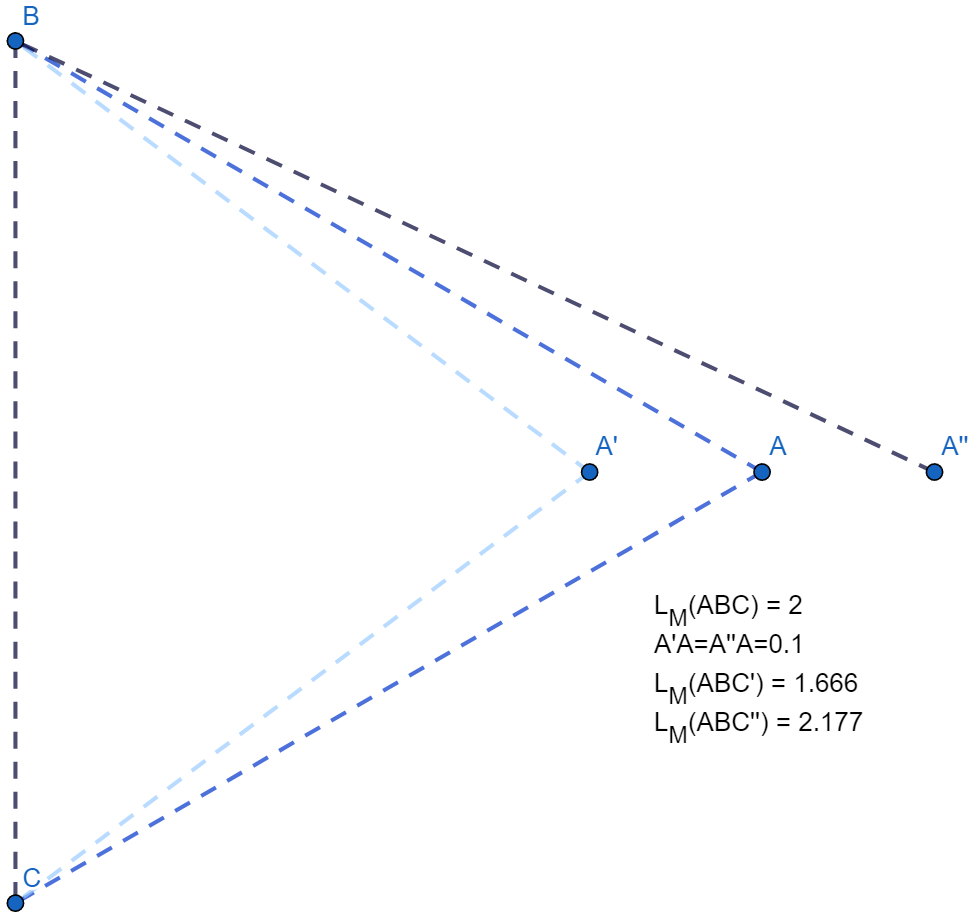
\includegraphics[scale=1.3]{plot9.png}
  \end{center}
  \caption{\label{fig:10}Visual explanation of local minimum property; as we change $A$ into $A'$ and $A''$, we decrease and increase $\operatorname{L_S}$ by 0.1, however we decrease $\operatorname{L_M}$ by 0.333 and increase it by 0.177, respectively.}
\end{figure}

Another observation is that in these local minima, most of the edges of the minimum spanning tree join in 60°. 

\subsubsection{Local minima of four terminals}
Figures \ref{fig:7}, \ref{fig:8} and \ref{fig:9} shows us various local minima of the $\operatorname{SR}$ function. Even in these cherry-picked examples, most of the full subcomponents (as defined in \cite{GP1968}) of the Steiner minimum tree are equilateral triangles. This subsection will attempt to explain the relative lack of 4 terminal full subcomponents and the properties of the  quadrilateral full subcomponent appearing in Figure \ref{fig:9}.

Based on only the first condition, we would expect rhombi with every possible angle to appear; for example, the square would be a local minimum. Thus, to determine the global minima of four terminals where no two terminals overlap, we have to find the global minimum of the rhombi.

To find the global minimum of the rhombi, without loss of generality let us assume that the rhombi have terminals at $A=(-x;0)$, $B=(0;1)$, $C=(x;0)$ and $D=(0;-1)$ as a function of $x$. Let us restrict the domain to $x\geq1$, as "squishing" the rhombus achieves the same shape "stretching" it, however some calculations do not work when squishing the rhombus. Thus, the length function the Steiner minimal tree in its most simplified form is:

\begin{equation}
  \label{eq:1}
  \operatorname{SMT_{rhombus}}(x)=2\sqrt{x^2+\sqrt{3}x+1}
\end{equation}

The minimum spanning tree is calculated as a piecewise function:

\begin{equation}
  \label{eq:2}
  \operatorname{MST_{rhombus}}(x)=  
  \begin{cases} 
    2+2\sqrt{x^2+1} & x >\sqrt{3} \\
    3\sqrt{x^2+1} & \text{otherwise} \\
  \end{cases}
\end{equation}

The derivation for both functions is shown in the Appendix. We can define the Steiner ratio function for rhombi as $\operatorname{SR_r}(x) = \frac{\operatorname{SMT_{rhombus}}(x)}{\operatorname{MST_{rhombus}}(x)}$. The singular global minimum of $\operatorname{SR_r}(x)$ is $x=\sqrt{3}$ and $\operatorname{SR_r}(\sqrt{3})=\frac{\sqrt{7}}{3}\approx 0.882$, as depicted in Figure \ref{fig:11}; Figure \ref{fig:12} shows us the actual set of terminals which give rise to the global minimum Steiner ratio.

\begin{figure}[h!]
  \begin{center}
  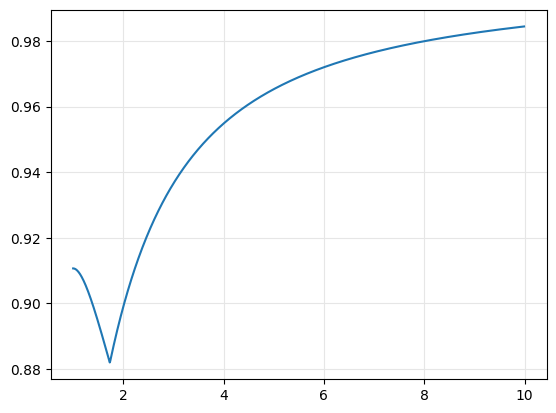
\includegraphics[scale=0.5]{plot10.png}
  \end{center}
  \caption{\label{fig:11} The first few places of $\operatorname{SR_{r}}$.}
\end{figure}

\begin{figure}[h!]
  \begin{center}
  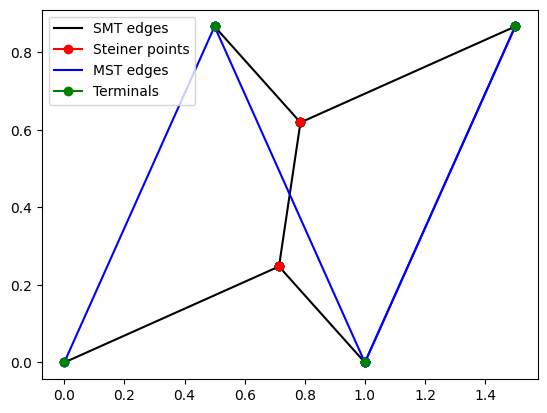
\includegraphics[scale=0.5]{plot11.png}
  \end{center}
  \caption{\label{fig:12} The set of terminals which produce the global minimum in Figure \ref{fig:11}.}
\end{figure}

The underlying rhombus which is formed at $\operatorname{SR_r}(x)$ has several other interesting properties and observations, including:
\begin{itemize}
  \item It is the breakpoint between the two possible weight-preserving isomorphic classes of spanning tree topologies, as discussed in the Appendix. %This means that we do not need to search for both categories' global minima to find 
  \item The terminals form two equilateral triangles which\\share a side, thus all possible edges join in 60°.
  \item Is (approximately) the same set of terminals as in the lower right corner of Figure \ref{fig:9}.
  \item The edges of the Steiner tree have a ratio of 1:2:1:2:1, with the longer Steiner tree edges are connected to $A$ and $C$. 
  \item Let $p_i$ be the Steiner point incident to terminal $s_i$ ($p_j=p_k$, is possible; $i,j,k \leq 4$), then $\sum\limits_{i=0}^4\overrightarrow{p_is_i}=(0;0)$. This applies to all rhombi.
\end{itemize}

Nevertheless, there are arrangements of four terminals that have a lower Steiner ratio; however, none of those are local minimum. From now on, let us call the global minimum of the rhombi the  \emph{pure} global minimum of the 4 terminal instances. 

For machine learning, the other rhombi are "false" minima, all the values in the Jacobian matrix of $operatorname{SR}(S)$, where $S$ are the terminals of a rhombus, are 0 and the Hessian matrix is negative\footnote{As possibly interpreted by an optimizer; the application of differentiation is looser for optimizers than as rigidly defined in mathematics.}. This suggests that optimizers that rely solely on Jacobians and Hessians are not suitable for optimizing $\operatorname{SR}(S)$.

\subsubsection{Local minima of n terminals}
We will now move on from 4 terminal instances into higher terminal instances. We do not see any 5 terminal full Steiner tree subcomponents in any of the Figures. If we continue the pattern started with the pure global minimum of the 4 terminal instances, i.e. put down a terminal down such that it forms an equilateral triangle with other two existing terminals\footnote{It does not matter next to which two terminals we put the new terminal; all configurations result in the same minimum spanning tree and Steiner minimum tree, rotated.}, we get the instance displayed in Figure \ref{fig:13}. Because the conjecture is proven for 5 terminals, we know that this must also be the pure global minimum of the 5 terminal instances; the same argument can be repeated for 7 terminals.

\begin{figure}[h!]
  \begin{center}
  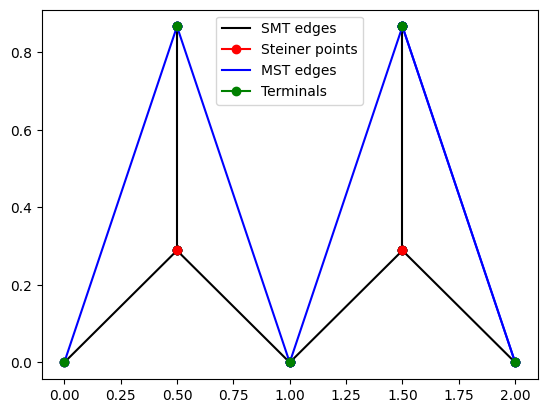
\includegraphics[scale=0.5]{plot12.png}
  \end{center}
  \caption{\label{fig:13} The set of terminals which produces the pure global minimum for 5 terminals.}
\end{figure}

Based on the experimental results from Section \ref{sec:ea}, we also conjecture that
\begin{conjecture}
  No 5 terminals which form a full Steiner minimum tree is the pure global minimum of the 5 terminal instances.
\end{conjecture}

Repeating the same process for 6 terminals, it now matters where we put the new terminal; we can either put it "on top" of the two triangles to form an equilateral triangle with sides double the original side's length, or we can put it to the "side", resulting in a zigzag or tooth shape. Putting it to the side results in a much lower Steiner ratio, as Figure \ref{fig:14} shows us. Using the method from \cite{uteshev2021length}, we get that the exact Steiner ratio is $\frac{\sqrt{19}}{5}$. It has analogous properties to the pure global minimum for 4 terminal instances:

\begin{itemize}
  \item The minimum spanning tree is a breakpoint between multiple weight-preserving isomorphic classes of spanning tree topologies. %This means that we do not need to search for both categories' global minima to find 
  \item The terminals form four equilateral triangles.
  \item Is (approximately) the same set of terminals as in the lower half of Figure \ref{fig:8}.
  \item The edges of the Steiner tree have a ratio of 1:2:3.
  \item Let $p_i$ be the Steiner point incident to terminal $s_i$ ($p_j=p_k$, is possible; $i,j,k \leq 6$), then $\sum\limits_{i=0}^6\overrightarrow{p_is_i}=(0;0)$. 
\end{itemize}


\begin{figure}[h!]
  \begin{center}
  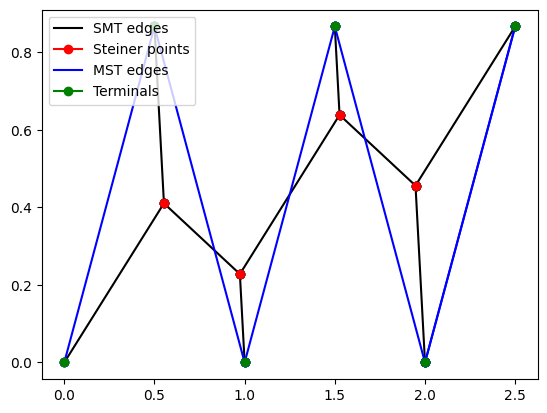
\includegraphics[scale=0.5]{plot13.png}
  \end{center}
  \caption{\label{fig:14} The conjectured set of terminals which produces the pure global minimum for 6 terminals; $\operatorname{SR}(S) = \frac{\sqrt{19}}{5}\approx 0.872$.}
\end{figure}

% conjecture: the steiner tree topology of these

Figure \ref{fig:15} shows us that if continue putting terminals to the side, all the relevant properties also hold for 50 terminals. Formalizing this,

\begin{definition}[Tooth set]
  Let the tooth set on $n$ terminals, or $T_n$ be the set of terminals such that each terminal $s_k$, $0\leq k \leq n-1$ has the coordinates $\left(\frac{k}{2}, \frac{k \bmod 2\sqrt{3}}{2}\right)$.
\end{definition}

Firstly, we conjecture that the Steiner tree patterns for $T_n$ we have seen so far continue as we put down more terminals:

\begin{conjecture}\label{c:1}
  For $T_{2k-1}$, $k\in\mathbb{Z}, k\geq 2$ the Steiner minimum tree topology is a series of $T_3$ topologies.

  For $T_{2k}$, $k\in\mathbb{Z}, k\geq 2$ the Steiner minimum tree topology is a full Steiner tree topology with Steiner points $p_0,\allowbreak p_1,\allowbreak \dots p_{2k-3}$, where $s_0$ and $s_1$ are connected to $p_0$ and $p_l, l\in\mathbb{Z}, 1\leq l\geq 2k-4$ is connected to $p_{l-1}, p_{l+1}, s_{l+1}$ and  $s_{2k-2}$ and $s_{2k-1}$ is connected to  $p_{2k-3}$. Furthermore,

    \begin{itemize}
    \item $\measuredangle(\overrightarrow{p_0s_0}, \overrightarrow{p_{2k-1}s_{2k-1}})=\pi$;
    \item $\measuredangle(\overrightarrow{p_0s_0}, \overrightarrow{p_{2l-1}s_{2l-2}})=\frac{2\pi}{3}, l\in\mathbb{Z}, 0\leq l\leq k-1$;
    \item $\measuredangle(\overrightarrow{p_0s_0}, \overrightarrow{p_{2l}s_{2l-1}})=\frac{5\pi}{3}, l\in\mathbb{Z}, 1\leq l\leq k$.
  \end{itemize}
\end{conjecture}

If Conjecture \ref{c:1} indeed holds (tests done with GeoSteiner shows us that it is true for $n\leq 100$), then the formula given by \cite{uteshev2021length} gives us

\begin{equation} \label{eq:4}
  \operatorname{L_S}(T_{2k}) = \sqrt{3k^2 -3k + 1}
\end{equation}

Derivation for Equation \ref{eq:4} is shown in the Appendix. From this, we can calculate the Steiner ratio of even-numbered $T_n$ as:

\begin{equation} \label{eq:5}
  \operatorname{SR}(T_{2k}) = \frac{\sqrt{3k^2 -3k + 1}}{2 k - 1}
\end{equation}

A consequence of Equation \ref{eq:5} is that interestingly $\allowbreak\lim\limits_{k=2}^\infty \allowbreak\operatorname{SR}(T_{2k})=\frac{\sqrt{3}}{2}$. Nevertheless, we even if Conjecture \ref{c:1} is not true, we know that $\operatorname{SR}(T_{2k})>\frac{\sqrt{3}}{2}$, because all terminals lie on a triangular lattice, and the Gilbert-Pollak conjecture is proven for sets of terminals triangular lattices \cite{po}.

Secondly, we conjecture that:

\begin{conjecture}\label{c:2}
  $T_n$ is the pure global minimum for $n$ terminals.
\end{conjecture}

For $n=3,4,5,7$ this is proven. The empirical evidence behind this is the fact that the only full Steiner subcomponents in the optimizer results are $T_n$ full subcomponents. Admittedly, only a few experiments with 10 terminals are presented; however, most of the optimizer results are similar to the ones presented, and optimizations runs for even 20 terminals take minutes to execute and a large portion of the experiments are not successful (meaning the iteration limit is reached or problems with numerical precision). Furthermore, if this conjecture holds, then we have proven the Gilbert-Pollak conjecture. 



% \operatorname{L_S}(T_{2k}) = \left|{\frac{3}{2} k + \frac{\sqrt{3}}{2} i k - 1}\right|


% TODO: remark maybe?
% \begin{proof}
%   Let us prove this by contradiction; for $2k=4$, we already proved that this is the Steiner minimum tree topology, so we will only be considering the cases $k\geq 3$.

%   Firstly, let us suppose that $\operatorname{SMT}(T_{2k})$ has a cherry that contains any terminals not included in $\{s_0, s_1, s_{2k-2}, s_{2k-1}\}$; let us denote the two terminal of the cherry $s_m$ and $s_u$. $\operatorname{len}(s_m, s_u) = 1$, because otherwise the lunes would overlap with one of the terminals. TODO: expand this
% \end{proof}

% \begin{lemma}[]
%   % For $T_{2k}$, $k\in\mathbb{Z}, k\geq 2$ let the $C_{2k}$ be the Steiner tree topology, where  $s_0$ and $s_1$, and $s_{2k-2}$ and $s_{2k-1}$, respectively, are on cherries and all other terminals 
%   For $T_{2k}$, $k\in\mathbb{Z}, k\geq 2$, let $p_l$ be the Steiner point incident to terminal $s_l$, then 
%   \begin{itemize}
%     \item $\measuredangle(\overrightarrow{p_0s_0}, \overrightarrow{p_{2k-1}s_{2k-1}})=\pi$;
%     \item $\measuredangle(\overrightarrow{p_0s_0}, \overrightarrow{p_{2l-1}s_{2l-1}})=\frac{2\pi}{3}, l\in\mathbb{Z}, 0\leq l\leq k-1$;
%     \item $\measuredangle(\overrightarrow{p_0s_0}, \overrightarrow{p_{2l}s_{2l}})=\frac{5\pi}{3}, l\in\mathbb{Z}, 1\leq l\leq k$.
%   \end{itemize}
% \end{lemma}
% TODO: visual explanation?
% \begin{proof}
%   Let us prove using total induction.
%   % vertical cherries are easy to handle
%   % horizontal cherries 
% \end{proof}
% The Steiner minimal trees depicted in Figures \ref{fig:12}, \ref{fig:14} and \ref{fig:15} all satisfy these conditions 

\section{Theoretical approaches}

In the literate review, we have seen four different proofs for lower bounds using the same technique - focusing on the cherry. Each proof lists a ``web of conditions'' that the cherry and nearby points must satisfy - which yields a lower bound less than $\frac{\sqrt{3}}{2}$. The problem with this approach is that we are trying to prove that the cherry itself makes the Steiner ratio to be at least $\frac{\sqrt{3}}{2}$, but we cannot prove that the Steiner ratio is more than  $\frac{\sqrt{3}}{2}$, as we can produce set of terminals with Steiner ratio arbitrarily close to $\frac{\sqrt{3}}{2}$ such that the Steiner tree contains a cherry. This means that  these set of conditions can only prove that the Steiner ratio is equal to  $\frac{\sqrt{3}}{2}$, and if there are any assumptions that are not strong enough, then not even the equality can be proven. Therefore, the web of conditions using cherries is unlikely to produce a proof of the conjecture; if we are to prove the conjecture, we need to come up with conditions that apply everywhere. The biggest problem here is that there are no easy-to-state and strong enough global properties that do not have exceptions and corner cases.


TODO: the need for global properties

\section{Conclusions}



\bibliographystyle{abbrv}
\bibliography{example}

\section{Appendix}

\begin{figure}[h!]
  \begin{center}
  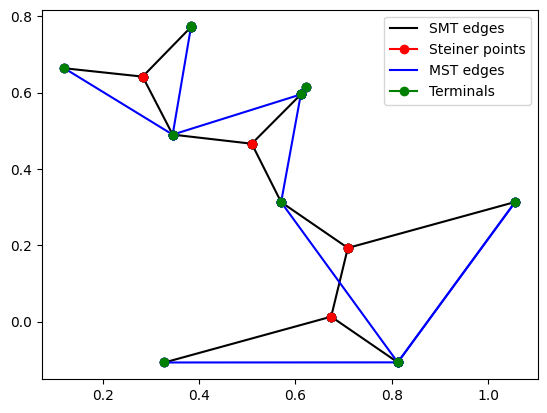
\includegraphics[scale=0.5]{plot8764.png}
  \end{center}
  \caption{\label{fig:9}10 random points optimized for $\operatorname{SR}(S)$ with SLSQP; $\operatorname{SR}(S)\approx 0.8764$}
\end{figure}

Alternative phrasings for Lemma \ref{l:1}:

\begin{lemma}
  Let $n$ be the number of terminals and let $S$ be an input vector for $\operatorname{SR}$. $\operatorname{SR}(S)$ is a local minimum if for every terminal, there exists at least two $\operatorname{MST}(S)$ topologies where the degree of the terminal is different.
\end{lemma}
\begin{lemma}
  Let $n$ be the number of terminals and let $S$ be an input vector for $\operatorname{SR}$. $\operatorname{SR}(S)$ is a local minimum if for every terminal $s_i$, $i\in\{1,2,\dots n\}$, there exists at least one $M=\operatorname{MST}(S)$ such that $M$ has at least one edge $s_is_m$, $m, k\in \in\{1,2,\dots n\}$ such that we can substitute $s_is_m$ with another edge $s_ks_m$  $m, k\in\{1,2,\dots n\}$ to produce $M'$, and the weight of $M$ and $M'$ are equal.
\end{lemma}

\begin{proof} [Derivation for Equation \ref{eq:1}:]

Firstly, we use the construction from provided Karl Bopp \cite{bopp} to find the length of the Simpson line and thus the Steiner minimum tree, where $P_1$ and $P_2$ are the Simpson points of the rhombus:
\[
  \operatorname{SMT_{rhombus}}(x) = \operatorname{len}(P_1P_2)
\]
This is expanded into:
\[
  = \sqrt{(x_{P_1}-x_{P_2})^2+(y_{P_1}-y_{P_2})^2}
\]
Without loss of generality, let us assume that the two terminals of the two cherries on the Steiner tree are $A$, $B$ and $C$, $D$ (every Steiner tree of these points have the same length). Therefore, $P_1$ is the point which satisfies $\operatorname{len}(P_1A)=\operatorname{len}(P_1B)=\operatorname{len}(AB)$ and is outside the rhombus, and vice versa for $P_2$ and $C$, $D$. Thus, the coordinates for $P_1$ are:
\[
  P_1 = \left(\frac{(-x)^{2} \pm \sqrt{3} (-x)}{2 (-x)}, \pm \frac{\sqrt{3} (-x)}{2} + \frac{1}{2}\right)
\]

The correct root is:

\[
  P_1 = \left(\frac{(-x)^{2} - \sqrt{3} (-x)}{2 (-x)}, - \frac{\sqrt{3} (-x)}{2} + \frac{1}{2}\right)
\]

Similarly, the correct root for $P_2$ is:

\[
  P_2 =\left(\frac{x^{2} + \sqrt{3} x}{2 x}, - \frac{\sqrt{3} x}{2} - \frac{1}{2}\right)
\]

If we plug the values of $P_1$ and $P_2$ into $\operatorname{SMT_{rhombus}}(x)$ and simplify the expression, we get:
\[
  \operatorname{SMT_{rhombus}}(x)=2\sqrt{x^2+\sqrt(3)x+1}
\]

% \begin{figure*}[h!]
%   \begin{center}\[
%     \sqrt{(\frac{(-x)^{2} - \sqrt{3} (-x)}{2 (-x)}-\frac{x^{2} + \sqrt{3} x}{2 x})^2+(- \frac{\sqrt{3} (-x)}{2} + \frac{1}{2}-(-\frac{\sqrt{3} x}{2} - \frac{1}{2}))^2}
%   \]
%   \end{center}
%   \end{figure*}
  

  
  
\end{proof}


\begin{proof} [Derivation for Equation \ref{eq:2}:]
  For the rhombus, for each instance there are three different weight-preserving isomorphic classes of spanning tree topologies:
  \begin{itemize}
    \item Three sides
    \item Two opposing sides and the $BD$ diagonal
    \item Two opposing sides and the $AC$ diagonal
  \end{itemize}
  The smallest weight of these trees is the minimum spanning tree of the rhombus. Because of our choice to restrict the domain to $[1;\infty]$, the third case can never happen. The formula for a side of the rhombus is $\sqrt{(\pm x-0)^2+(0\mp 1)^2}$, which can be simplified into $\sqrt{x^2+1}$, and the length of the diagonal is 2, thus the formulae for the trees are
  \begin{itemize}
    \item $3\sqrt{x^2+1}$
    \item $2+2\sqrt{x^2+1}$
  \end{itemize}
  Now we have to find the solutions for $$3\sqrt{x^2+1} < 2+2\sqrt{x^2+1}$$  to determine the places where the second  category of topologies is better than the first category. The solution is $x<-\sqrt{3}$ or $x>\sqrt{3}$, giving us
\[
  \operatorname{MST_{rhombus}}(x)=  
\begin{cases} 
  2+2\sqrt{x^2+1} & x >\sqrt{3} \\
  3\sqrt{x^2+1} & \text{otherwise} \\
\end{cases}
\]
\end{proof}
\begin{figure}[h!]
  \begin{center}
  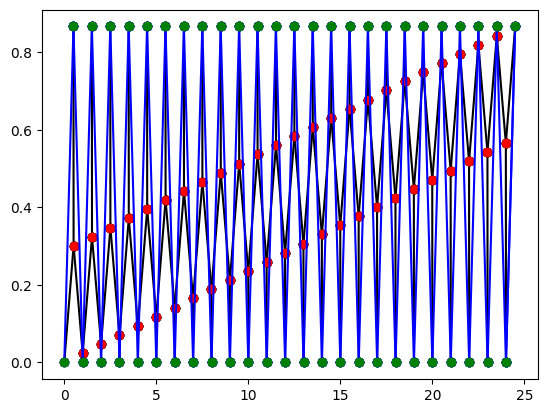
\includegraphics[scale=0.5]{plot14.png}
  \end{center}
  \caption{\label{fig:15} The conjectured set of terminals which produces the pure global minimum for 50 terminals; $\operatorname{SR}(S) \approx \frac{\sqrt{3}}{2}$.}
\end{figure}

% \begin{figure*}
%   \begin{center}
%     \begin{equation} \label{eq:4}
%       \operatorname{L_S}(T_{2k}) = \left|{k + \left(\frac{\sum_{m=1}^{2 k - 2} \left(- \left(-1\right)^{\frac{2}{3}} m + \left(\sqrt[6]{-1} \sqrt{3} \left(m \bmod 2\right)\right)\right) \left(e^{i \pi \left(\left(m + 1\right) \bmod 2\right)}\right)}{2}\right) - \frac{1}{2} + \frac{\sqrt{3} i}{2}}\right|
%     \end{equation}
%   \end{center}
% \end{figure*}
\begin{proof}[Derivation for Equation \ref{eq:4}]
  Let us use the formula from \cite{uteshev2021length}; to do so let $T_n$ be not a set of terminals on a Euclidean plane but a set of complex numbers (with the same values and everything defined analogously). Let the "base" vector be $\overrightarrow{p_0s_0}$. Then, we need to calculate each orientation of $\overrightarrow{p_js_k}$; because we assumed Conjecture \ref{c:1} holds, we have four cases:
  \begin{enumerate}
    \item The base orientation, $s_0=(0+0i)$;
    \item $s_{2k-1}$, we have to multiply by $(\cos{\pi}+\sin{\pi}i)$;
    \item $s_{2l-2}$, we have to multiply by $(\cos{\frac{2\pi}{3}}+\sin{\frac{2\pi}{3}}i)$;
    \item ${2l-1}$, we have to multiply by $(\cos{\frac{5\pi}{3}}+\sin{\frac{5\pi}{3}}i)$.
  \end{enumerate}
  Furthermore, because we have an even number of terminals, cases 3 and 4 come in pairs
\end{proof}
% \frac{k \bmod 2\sqrt{3}}{2}

\end{document}
